% !TeX encoding = macintosh
\documentclass{beamer}
\usepackage[italian]{babel}
\usepackage[applemac]{inputenc}
\usetheme{metropolis}           % Use metropolis theme
\usepackage{graphicx}
\usepackage{amsmath,amssymb}
\usepackage{tikz}
\usepackage{listings}
\usepackage{algorithm2e}
\usepackage{float}
\usepackage{xcolor}
\usepackage[export]{adjustbox}
\usepackage[absolute,overlay]{textpos}
\newcommand*{\redcolor}{red}
\makeatletter
\newcommand{\boxedred}[1]{\textcolor{\redcolor}{%
		\fbox{\normalcolor\m@th$\displaystyle#1$}}}
\makeatother	
\newcommand*{\greencolor}{darkgreen}
\makeatletter
\newcommand{\boxedgreen}[1]{\textcolor{\greencolor}{%
		\fbox{\normalcolor\m@th$\displaystyle#1$}}}
\makeatother	
\graphicspath{{./img/}}
\newcommand{\norm}[1]{\left\lVert#1\right\rVert}
\usepackage{color}
\definecolor{lightgray}{rgb}{.9,.9,.9}
\definecolor{darkgray}{rgb}{.4,.4,.4}
\definecolor{purple}{rgb}{0.65, 0.12, 0.82}
\definecolor{darkgreen}{rgb}{0.14, 0.62, 0.19}

\newcommand\tab[1][1cm]{\hspace*{#1}}

\title{Design and simulation of Geyser explosions through Computer Graphics}
\date{08/06/2017}
\author{Francesco Lombardi, Alessandro Sestini}
\institute{Universit� degli Studi di Firenze\\Dipartimento di Ingegneria dell'Informazione\\\\\\Computer Graphics \& 3D
}
%\titlegraphic{
\includegraphics[width=0.2\textwidth]{stemma}}
\begin{document}
 %\maketitle
  
  \begin{frame}[noframenumbering,plain]
	\tikz [remember picture,overlay]
	\node at
	([shift=({4cm,3.1cm})]current page.south)
	%or: (current page.center)
	{
\includegraphics[width=0.25\textwidth]{stemma}};
	\maketitle
\end{frame}

\begin{frame}[plain]{Indice}
	\setbeamertemplate{section in toc}[sections numbered]
	\tableofcontents[hideallsubsections]
\end{frame}

\section{Introduction}

\begin{frame}{Introduction}

\begin{block}{Idea}
	Realization of Geyser's natural phenomenon caused by a water explosion through WebGL and Three.js technologies.
\end{block}

\fbox{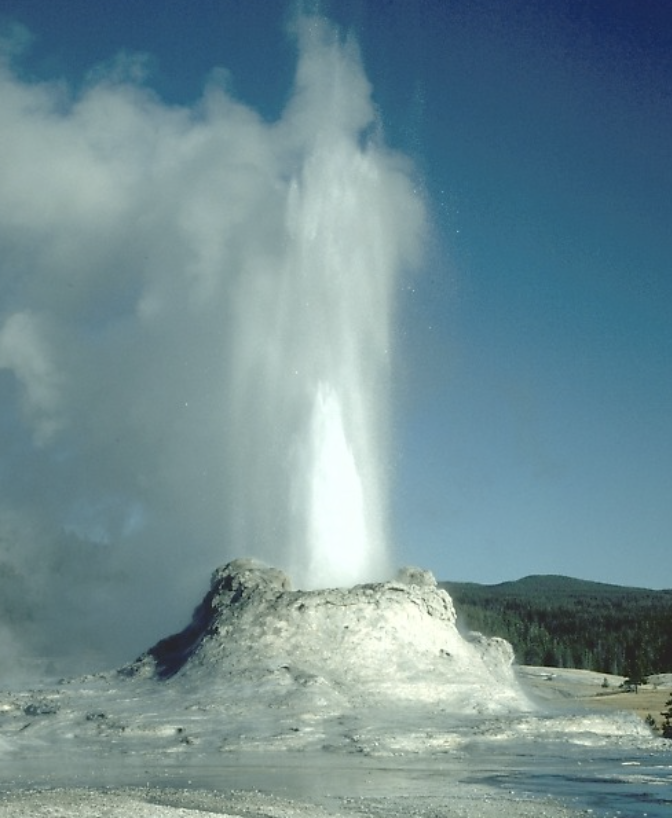
\includegraphics[width=.6\textwidth,height=5.5cm]{esplosione}}
\centering
\end{frame}

\begin{frame}{Introduction}
	\begin{block}{Project Aim}
		\begin{itemize}
			\item Simulation of the \textbf{physics} of water and steam particles
			\item Description of the motion of water particles following a \textbf{parabolic trajectory}
			\item Description of the \textbf{randomic} motion of steam particles in 3D space
			\item Creation of a pseudo-realistic scene
		\end{itemize}
	\end{block}
\end{frame}

\section{Scene}

\begin{frame}{Scene}
\begin{block}{Environment Building}
	\begin{itemize}
		\item Creation of a \textbf{cubeGeometry} with different textures for each face
		\item Rendering back-face culling: \textbf{back-side}
		\item Creation of the \textbf{cubic ground} applying a unique texture for all faces 
	\end{itemize}
\end{block}
\end{frame}

\begin{frame}{Scene}
\begin{block}{Lights and Materials}
		\begin{itemize}
		\item Application of a white \textbf{Ambient Light}
		\item Addition of a \textbf{Spot Light} simulating sun light
		\item Application of a \textbf{Shiny} material to the ground in order to reflect incoming light
	\end{itemize}
\fbox{\includegraphics[width=.6\textwidth,height=4cm]{lightHelper}}
\centering
\end{block}
\end{frame}

\begin{frame}{Scene}
\begin{block}{Water Mirror}
\begin{itemize}
	\item Realization of reflecting water through Three.js library with a custom shader 
\end{itemize}
\fbox{\includegraphics[width=.6\textwidth,height=4cm]{water}}
\centering
\end{block}
\end{frame}

\section{Physics}

\begin{frame}{Physics}
\begin{block}{Particles Creation (for both water and steam)}
	Mapping particles position in 2D space by:
	\begin{itemize}
		\item Splitting a \textbf{Gaussian Function} along y-axis in sub-intervals creating concentric circles in the xz-plane
	\end{itemize}
	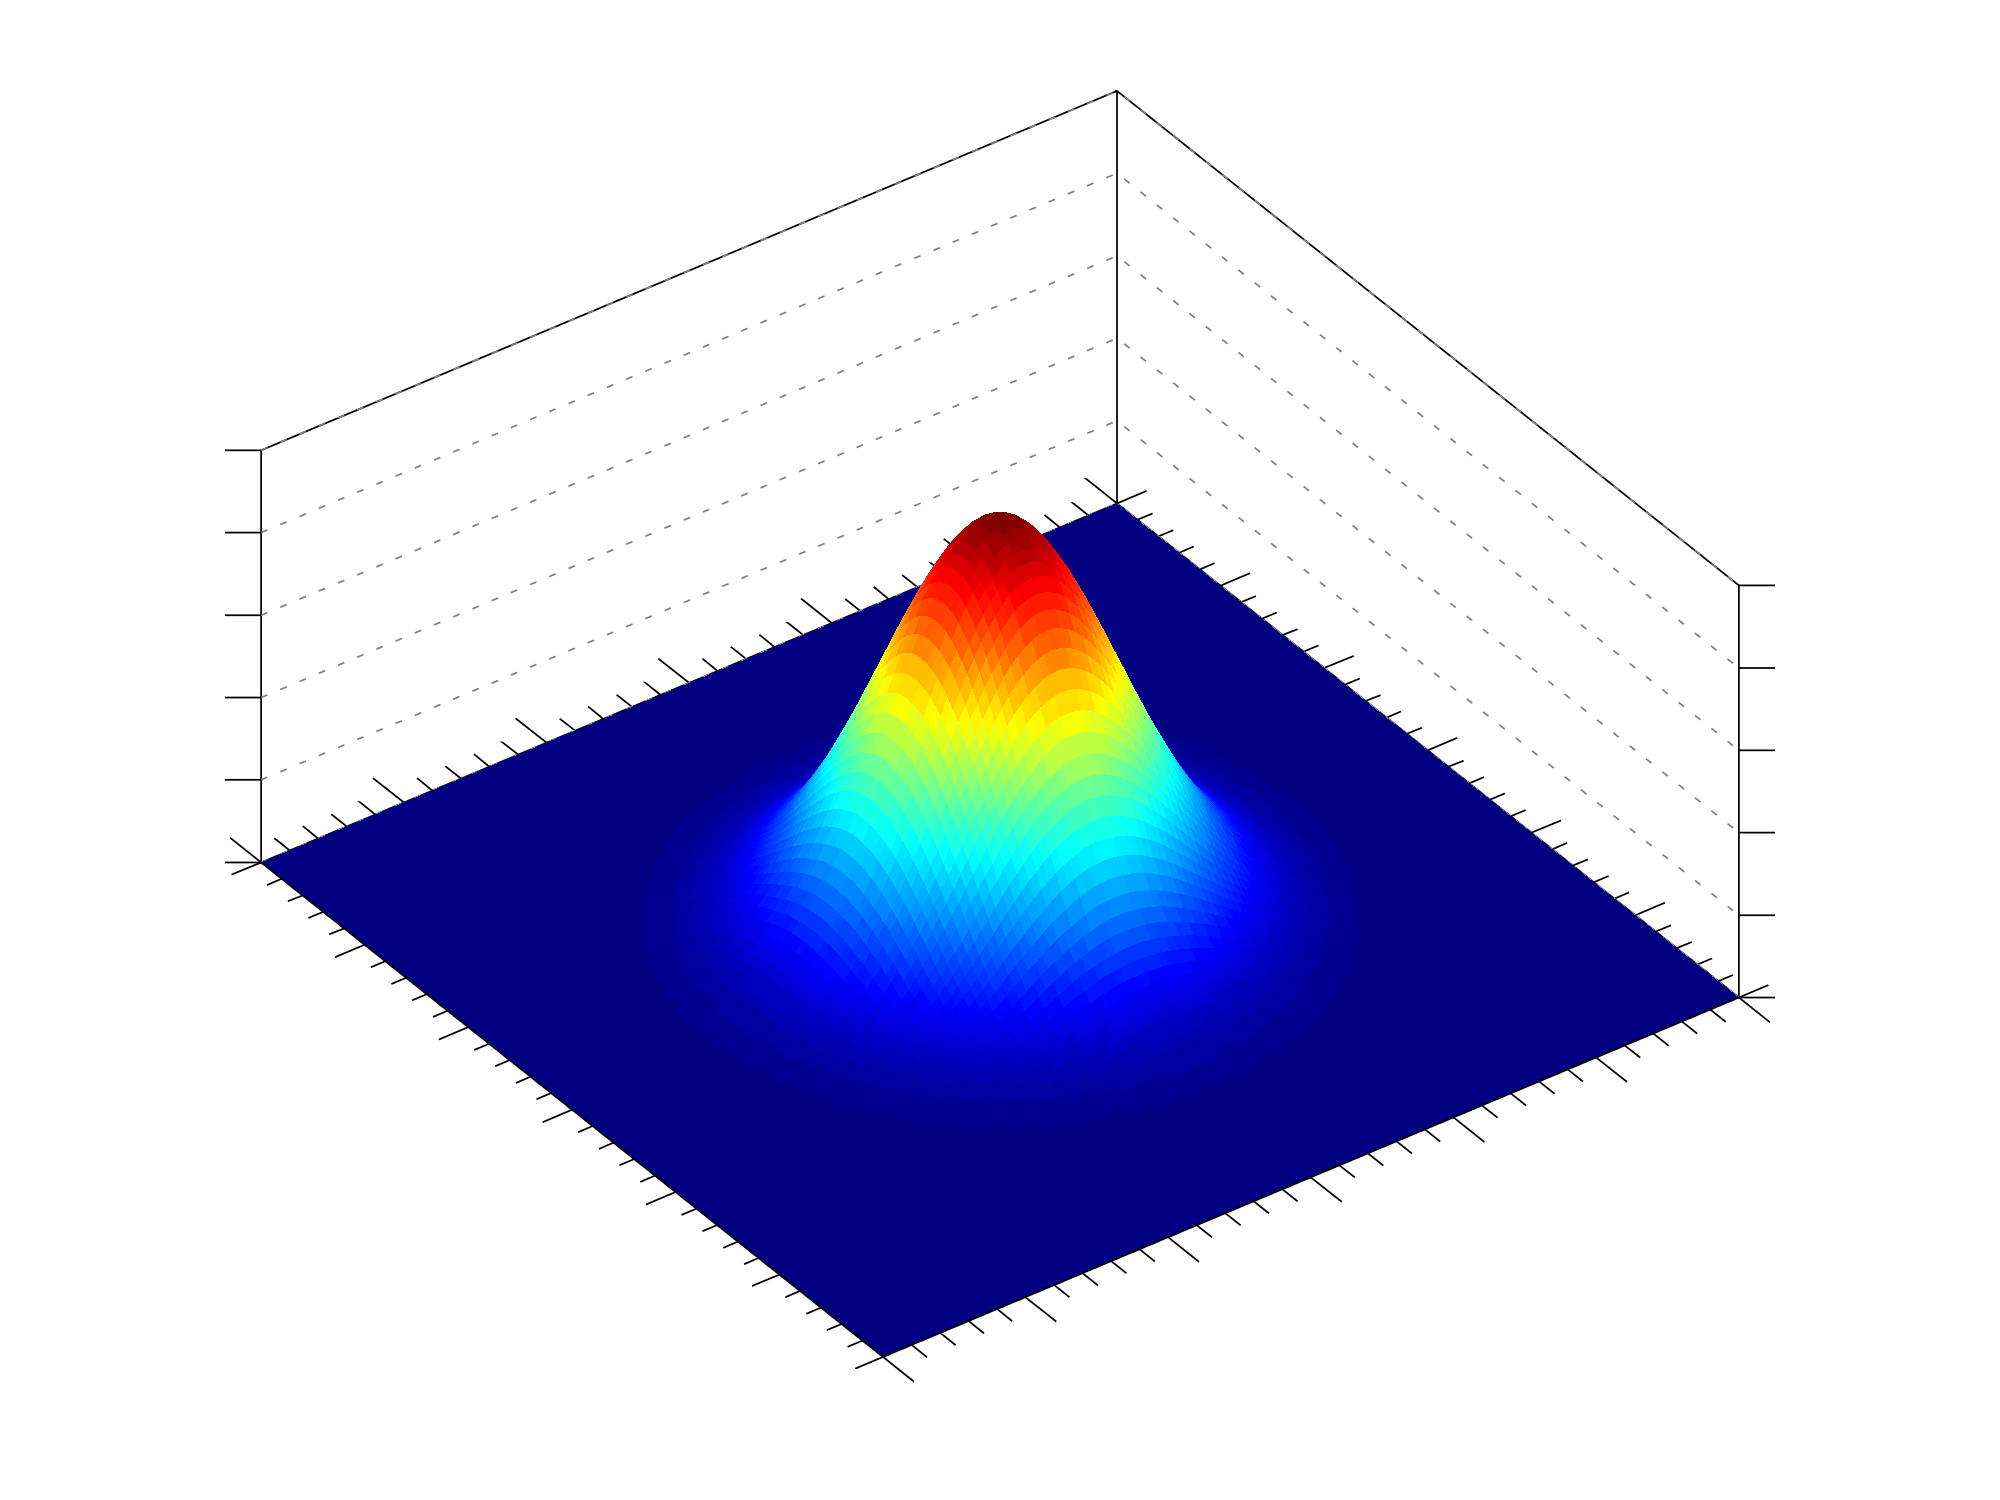
\includegraphics[width=.7\textwidth,height=5.5cm]{Gaussian.png}
	\centering
\end{block}
\end{frame}

\begin{frame}{Physics - Particles Creation}

	\begin{itemize}
		\item  Arranging points in \textbf{random positions} all over the circles following the relation:
		\begin{equation*}
		\begin{cases}
		x=R\,cos(\theta)\\z=R\,sin(\theta)
		\end{cases}
		\end{equation*}
		\item Pushing the xyz-coordinates in 2 different \textbf{Attribute Buffers} that are transferred to the shaders
	\end{itemize}
	\fbox{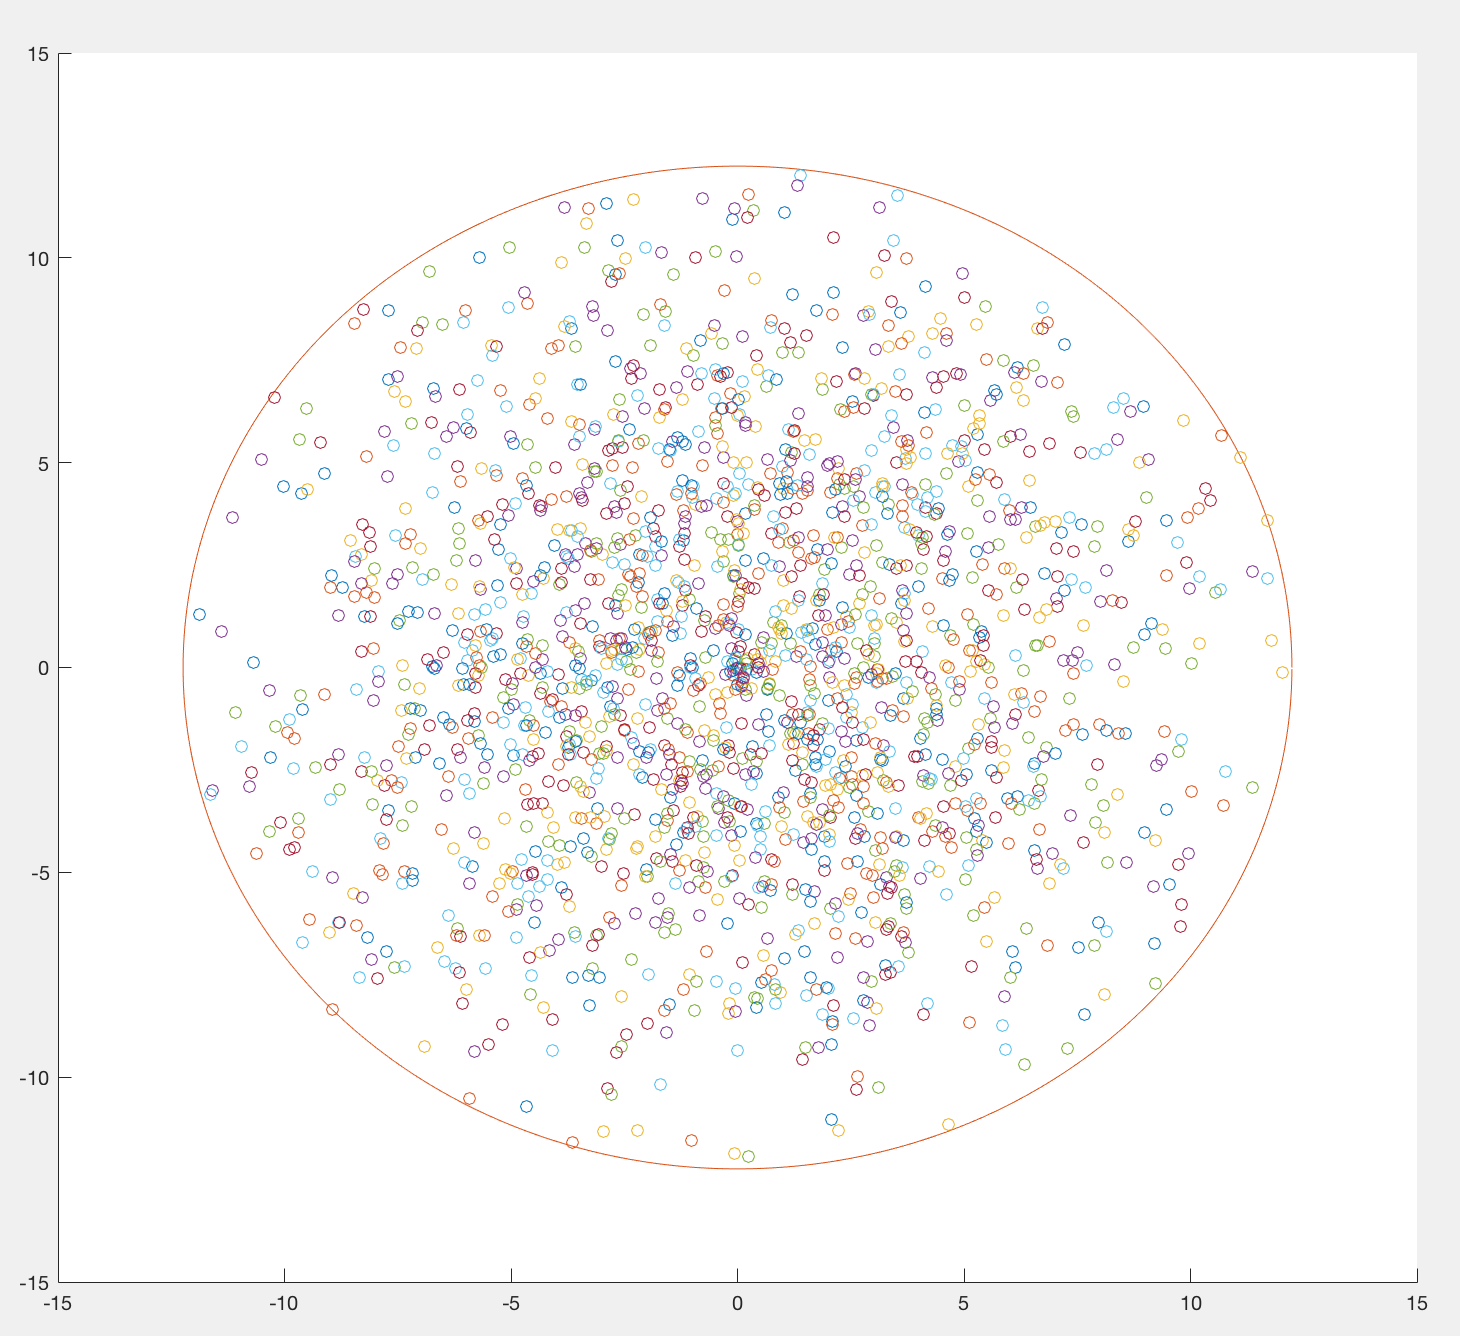
\includegraphics[width=.35\textwidth,height=3.5cm]{PointDistribution}}
	\centering

\end{frame}

\begin{frame}{Physics - Particles Creation}

\begin{itemize}
	\item Creating another Attribute Buffer with:
	\begin{itemize}
		\item random value \textbf{v0y} for the initial speed along the y-axis
		\item random value \textbf{v0r} for the initial speed along the xz-plane
		\item the \textbf{radial direction} for each water particle in the xz-plane, given by the angle $\theta$ seen before
		\item the direction for each steam particle in the xz-plane, given by a random value\textbf{ between $\omega \in [0, 2\pi]$}
	\end{itemize} 
\end{itemize}

\end{frame}

\begin{frame}{Physics - Particles Creation}

	\begin{itemize}
		\item Creating \textbf{Uniform Variables} for each type:
		\begin{itemize}
			\item \textbf{time} value t, inizialized to 0
			\item \textbf{texture} images 
			\item default value of \textbf{opacity}
			\item default value of \textbf{dimension}
		\end{itemize} 
	\end{itemize}

\end{frame}


\begin{frame}{Physics}
	
	\begin{block}{Vertex Shader - Water}
		\begin{itemize}
			\item Attribute Vector3 for initial \textbf{positions} ($x$, $y$ and $z$) and \textbf{movements} ($v0y$, $v0r$ and $\theta$)
			\item Uniform \textbf{float t} for time and uniform \textbf{float pointDim }for all particle dimensions
			\item The new position of a particle is computed following the law of \textbf{projectile motion}, with time value t upgraded every frame:
			\begin{itemize}
				\item \textbf{costant} speed in the xz plane 
				\item uniformly \textbf{accelerated} motion along the y axis 
			\end{itemize}
			\begin{equation*}
			\begin{cases}
			x(t) = v0r*cos(\theta)*t + x_0\\z(t) = v0r*sin(\theta)*t + z_0\\y(t) = -1/2*g*t^2 + v0y*t + y_0
			\end{cases}
			\end{equation*}
		\end{itemize}
	\end{block}

\end{frame}


\begin{frame}{Physics - Vertex Shader - Water}

\begin{block}{Code}
	\fbox{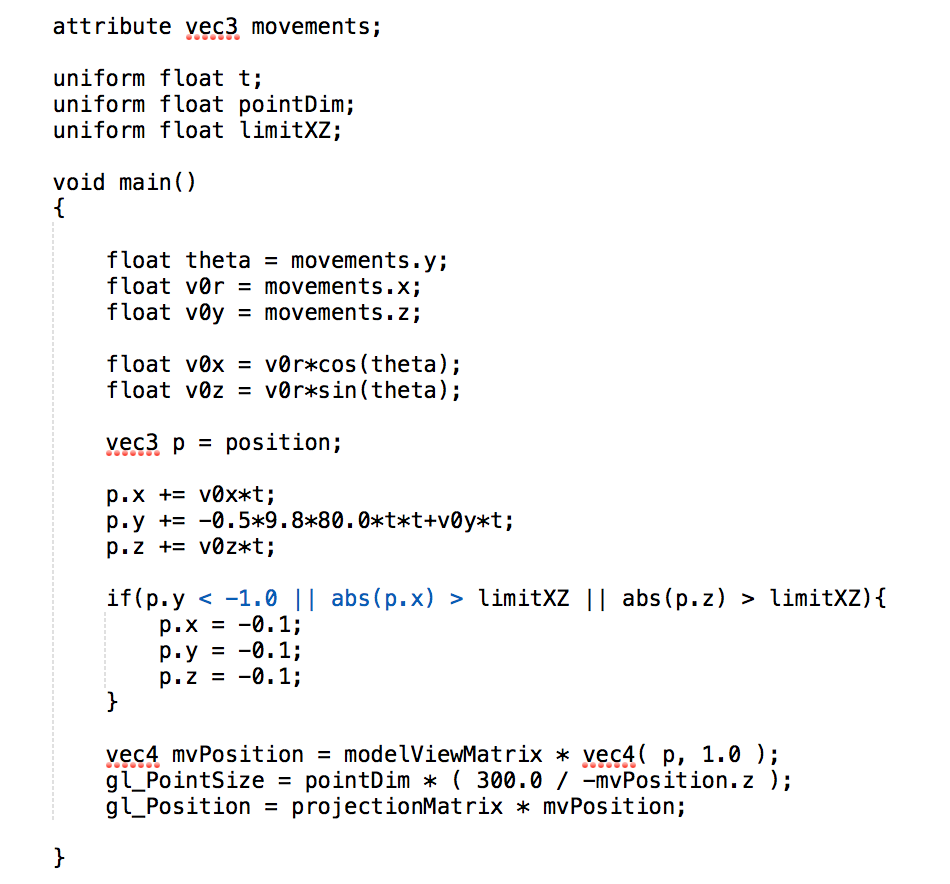
\includegraphics[width=.7\textwidth,height=7cm]{VertexShaderWater}}\centering
\end{block}

\end{frame}


\begin{frame}{Physics}

\begin{block}{Vertex Shader - Steam}
	\begin{itemize}
		\item Like water particles, same Vector3 for inital \textbf{positions} ($x,y$ and $z$) and same Vector3 for \textbf{movements} ($v0y, v0r$ and $\omega$)
		\item Same uniform  variables for \textbf{time} and point \textbf{dimensions}
		\item The new position of a particle is computed following a \textbf{costant motion} in all 3 directions

		\begin{equation*}
		\begin{cases}
		x(t) = v0r*cos(\omega)*t + x_0\\z(t) = v0r*sin(\omega)*t + z_0\\y(t) = v0y*t + y_0
		\end{cases}
		\end{equation*}

	\end{itemize}
\end{block}

\end{frame}


\begin{frame}{Physics - Vertex Shader - Steam}

\begin{block}{Code}
	\fbox{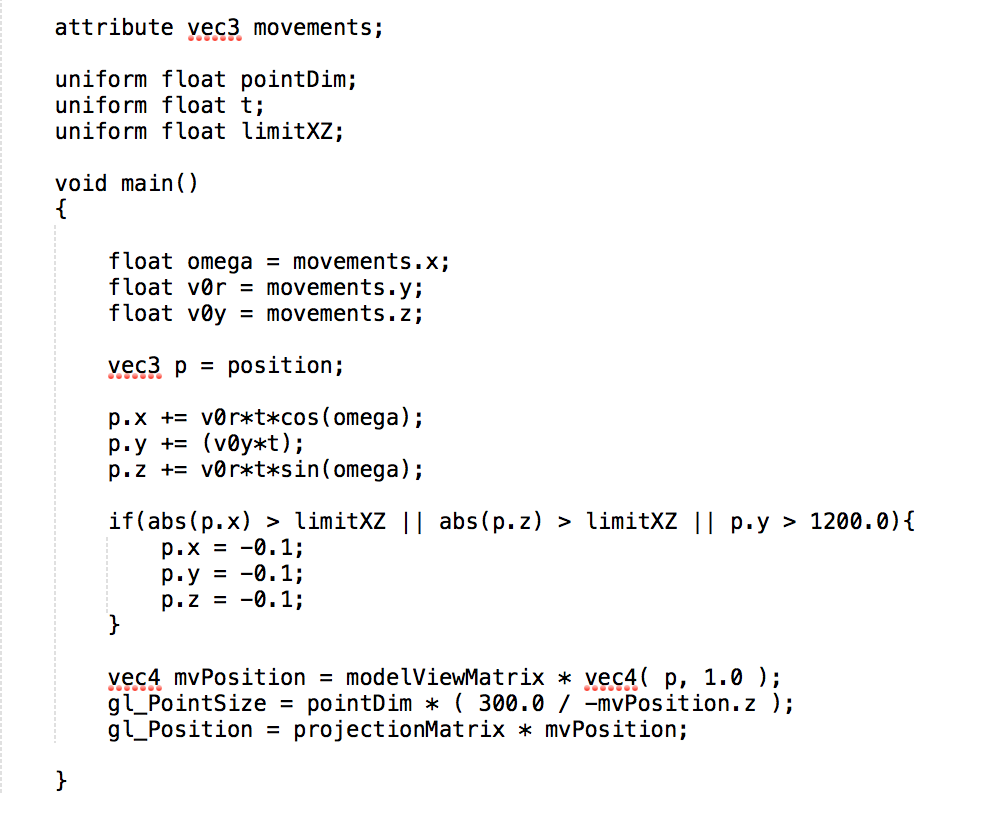
\includegraphics[width=.73\textwidth,height=7cm]{VertexShaderSteam}}\centering
\end{block}

\end{frame}


\begin{frame}{Physics}

\begin{block}{Fragment Shader}
	\begin{itemize}
		\item Same fragment shader for each type
		\item Only uniform variables for \textbf{textures} and \textbf{opacity} are defined
		\item If the value of opacity is set to 0, then \textbf{discard} the points
	\end{itemize}
\end{block}

\end{frame}

\begin{frame}{Physics - Fragment Shader}

\begin{block}{Code}
	\fbox{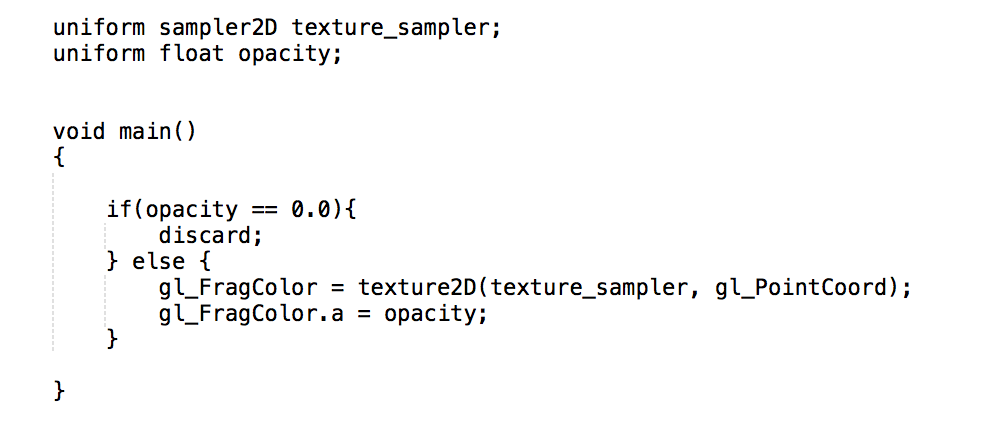
\includegraphics[width=1\textwidth,height=5cm]{FragmentShader}}\centering
\end{block}

\end{frame}

\begin{frame}{Physics}
\begin{block}{Texture}
	\begin{itemize}
		\item \textbf{Rounded textures} are used to simulate the effect of a more complex mesh
		\item \textbf{Additive Blending} technique is used to make the greater density areas gradually more white
	\end{itemize}
	\fbox{
\includegraphics[width=.3\textwidth,height=3cm]{water_drop}}
	\fbox{
\includegraphics[width=.3\textwidth,height=3cm]{steam_drop}}
	\centering
\end{block}
\end{frame}

\begin{frame}{Physics }

	\begin{block}{Render}
		When the space button is pressed, the render function distributes particles in the scene:
		\begin{itemize}
			\item particles movement is simulated by\textbf{ upgrading the uniform variable t} in every frame and computing the new position for each point
			\item \textbf{new particles are created} frame by frame (so with t inizialized to 0) and they are 'exploded'
			\item the process is \textbf{repeated} until a threshold value is reached
		\end{itemize}
	\end{block}

\end{frame}

\begin{frame}{Physics }

\begin{block}{Physics Controls}
	Some controls have been implemented in order to let the users be able to customize their experience:

	\fbox{\includegraphics[width=.42\textwidth,height=5.0cm]{controls}}
	\centering
\end{block}

\end{frame}

\begin{frame}[noframenumbering,plain]
\tikz [remember picture,overlay]
\node at
([shift=({4cm,3.1cm})]current page.south)
%or: (current page.center)
{
\includegraphics[width=0.25\textwidth]{stemma}};
\maketitle
\end{frame}


\end{document}